\clearpage{\pagestyle{empty}\cleardoublepage}

\chapter{La fluorescenza}

\begin{flushright}\begin{small}\textit{"The beginning of knowledge\\
 is the discovery of something\\ we do not understand."}\\
- Frank Herbert -\\
\end{small}\end{flushright}

Questo capitolo si propone di descrivere il fenomeno della fluorescenza e come questo possa essere sfruttato nella marcatura di elementi biologici specifici.


\section{Cenni storici}

La fotoluminescenza è il processo con cui una sostanza assorbe fotoni provenienti da una determinata sorgente per poi riemetterli ad una lunghezza d'onda maggiore (shift di Stokes). 
Tale fenomeno prende il nome di \textit{fluorescenza} nel caso in cui la riemissione sia istantanea (tempi di emissione dell'ordine dei nanosecondi) e di \textit{fosforescenza} nel caso in cui la riemissione avvenga con tempi maggiori. 

Le prime osservazioni di fotoluminescenza risalgono al Seicento, quando l'alchimista dilettante Vincenzo Casciarolo trovò sui colli bolognesi, ai piedi del Monte Paderno, una pietra con la proprietà di trattenere la luce solare e riemetterla dopo un certo intervallo di tempo. 
Tale processo, non essendo immediato, può essere classificato come processo fosforescente di tipo inorganico. 
La pietra, inizialmente considerata magica, è nota come ``pietra di Bologna''; essa è costituita da barite ($BaSO_4$), un minerale che, una volta calcinato nel carbone, si trasforma in solfuro di bario ($BaS$), avente proprietà fosforescenti. 

Per quanto riguarda la fluorescenza, le prime osservazioni vennero fatte solo agli inizi dell'Ottocento da David Brewster e John F. W. Herschel. Brewster nel 1833 notò che quando un raggio di luce penetrava in una soluzione alcolica contenente clorofilla appariva di colore rosso, mentre nel 1845 Herschel osservò che una soluzione incolore di solfato di chinina sviluppava un colore blu quando esposta alla luce solare. 
Tuttavia per poter parlare effettivamente di fluorescenza bisogna aspettare il 1852, quando lo scienziato inglese Sir G. G. Stokes coniò il termine nel suo famoso lavoro ``On the Change of the Refrangibility of Light''. 
Al suo interno Stokes descrisse ed interpretò le osservazioni da lui fatte sul minerale fluorite ($CaF_2$): se illuminato con luce di eccitazione ultravioletta riemetteva in modo istantaneo radiazione appartenente al rosso. 
Ricerche successive permisero poi di capire che molti materiali come minerali, cristalli, vitamine, oli, resine e composti organici posseggono proprietà fluorescenti se irraggiati con luce ultravioletta. 

Nel primo decennio del Novecento Heimstädt e Lehmann svilupparono il primo microscopio a fluorescenza con il quale studiarono batteri, tessuti animali e vegetali.
Tuttavia, l'applicazione della fluorescenza al campo della biologia animale tardò ad essere sviluppata a causa della fluorescenza assai ridotta presentata da cellule e tessuti animali \cite{storia}.
Per ovviare a ciò, Max Haitinger nel 1933 introdusse l'uso della fluorescenza secondaria nello studio dei preparati biologici.
La sua idea presupponeva l'utilizzo di sostanze, dette fluorocromi o fluorofori, in grado di suscitare fluorescenza anche a concentrazioni bassissime (circa $10^{-6}$\%) e, pertanto, non in grado di danneggiare il preparato. 
In tal modo fu possibile marcare tessuti, batteri ed altri bersagli biochimici con alta specificità.
Il valore del microscopio a fluorescenza è stato significativamente dimostrato nel 1950 quando Coons e Kaplan riuscirono a localizzare antigeni specifici in tessuti in seguito a reazione con anticorpi marcati con il colorante fluoresceina.

Oggi la microscopia a fluorescenza è uno strumento fondamentale per le scienze biologiche e biofisiche ma ampiamente impiegato anche nello studio dei materiali, grazie ad alcune applicazioni che non sono ottenibili con nessuna delle altre tecniche di microscopia oggi esistenti. 
La possibilità di utilizzare nello stesso esperimento una molteplicità di fluorofori permette di individuare le cellule ed i componenti subcellulari con un alto grado di specificità, sino a riuscire a rivelare la presenza di una singola molecola, e di identificare più molecole bersaglio contemporaneamente.
Quest'ultima particolarità è molto importante in quegli esperimenti che mirano alla scoperta delle correlazioni esistenti tra i diversi meccanismi biochimici che si verificano all'interno delle cellule.


\section{Il fenomeno della fluorescenza}

Quando le cellule vengono attraversate da un fascio di luce laser di determinata frequenza ed intensità, fanno sì che quest'ultimo possa venire trasmesso, rifratto o, nel particolar caso in cui le molecole eccitate presentino proprietà emissive, riemesso come fotoluminescenza. 

Come visto, la fotoluminescenza è quel fenomeno per cui una molecola colpita da radiazione luminosa ad una certa lunghezza d'onda (frequenza di eccitazione) ne emette un'altra a lunghezza d'onda superiore (frequenza di emissione). 
Infatti, in seguito a questo assorbimento d'energia gli elettroni degli orbitali più esterni si spostano da un livello energetico ad uno superiore (eccitazione) instabile, la cui vita media è dell'ordine dei miliardesimi di secondo; successivamente gli elettroni tornano al livello energetico originario liberando solitamente l'energia assorbita sotto forma di radiazione elettromagnetica (emissione di fotoni). 
Poiché la resa energetica non è mai del 100\%, la radiazione liberata è di lunghezza d'onda superiore, e quindi di energia minore, rispetto a quella di eccitazione. 
Di conseguenza la radiazione di emissione, rispetto quella di eccitazione, risulta spostata verso la regione del rosso. 
Ciò conferisce a tali molecole una delle loro fondamentali proprietà, il cosiddetto spostamento di Stokes (``Stokes' shift'', \figurename~\ref{fig:stokes}), che rappresenta la differenza tra la lunghezza d'onda della luce emessa e quella della luce assorbita, ovvero, in modo analogo, tra l'energia del fotone di eccitazione e quella del fotone di emissione.
Questa proprietà è caratteristica di ogni molecola ed è limitata di solito a poche decine di nanometri.

\begin{figure}
 \centering
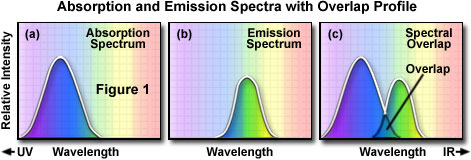
\includegraphics[scale=0.80]{img/CAP1stokes.jpg}
 \caption{ \small{Shift di Stokes.} In figura (a) si trova lo spettro di eccitazione incidente sul fluoroforo; in figura (b) lo spettro di emissione del fluoroforo; in figura (c) i due spettri sono mostrati sovraimposti, per evidenziare come vi sia una sovrapposizione fra i due.}
 \label{fig:stokes}
\end{figure}

Una volta che la molecola ha assorbito la radiazione incidente, si trova in uno degli stati vibrazionali di un livello energetico eccitato. 
Essendo soggetta a collisioni con le molecole circostanti, rilascia parte della sua energia sotto forma non radiativa, scendendo nella scala dei livelli vibrazionali interni allo stato eccitato. 
A questo punto, a seconda dell'intorno molecolare, la molecola può ritornare al suo stato fondamentale seguendo uno dei due seguenti processi:
\begin{description}
 \item [Processo non radiativo:]
Se le molecole circostanti sono in grado di assorbire la restante energia elettronica della molecola eccitata, quest'ultima completa il suo rilassamento in modo non radiativo, con conseguente liberazione di calore. 
Ciò permette alle molecole circostanti di attivare gradi di libertà vibrazionali, rotazionali e traslazionali, e perciò, come effetto complessivo, si ha un aumento dell'energia termica.
 \item [Processo radiativo:]
Se le molecole circostanti non sono in grado di assorbire la restante energia allora la molecola subisce un decadimento radiativo, ossia l'energia in eccesso viene liberata sotto forma di fotoni, aventi energia minore rispetto a quella dei fotoni che hanno causato l'eccitazione. 
Tale processo dà luogo ad un evento di emissione spontanea che può essere, a seconda dei casi, fluorescenza o fosforescenza.
\end{description}
La distinzione tra fluorescenza e fosforescenza fu originariamente fatta in base al tempo di vita della radiazione: nella fluorescenza la luminescenza cessa quasi subito dopo aver eliminato la radiazione eccitante, mentre nella fosforescenza la radiazione continua ad essere emessa, almeno per un breve lasso di tempo, anche dopo aver eliminato la sorgente eccitante. 
Infatti i materiali fluorescenti cessano di essere luminosi al cessare dello stimolo che ne determina la luminosità, mentre nei materiali fosforescenti la luce continua ad essere emessa per un certo periodo dopo la fine dello stimolo.

Con l'avanzare degli studi in tale ambito, si scoprì una più profonda distinzione tra i due fenomeni, legata alla natura degli stati elettronici coinvolti nelle transizioni responsabili dell'emissione di radiazione.
Quando un elettrone viene promosso da uno stato fondamentale, solitamente di singoletto, ($S_0$) ad uno eccitato, esso può mantenere lo spin originario oppure invertirlo: se l'eccitazione avviene con ritenzione dello spin si parla di stato di singoletto ($S_1$), se invece il passaggio allo stato attivato avviene con inversione dello spin si parla di stato di tripletto ($T_1$) (\figurename~\ref{fig:spin}). 
Allo stato di singoletto compete un'energia più alta e una vita media che va da $10^{-11}$ s a $10^{-9}$ s, mentre lo stato di tripletto ha energia inferiore e vita media che va da $10^{-3}$ s a $10^{1}$ s.

\begin{figure}
 \centering
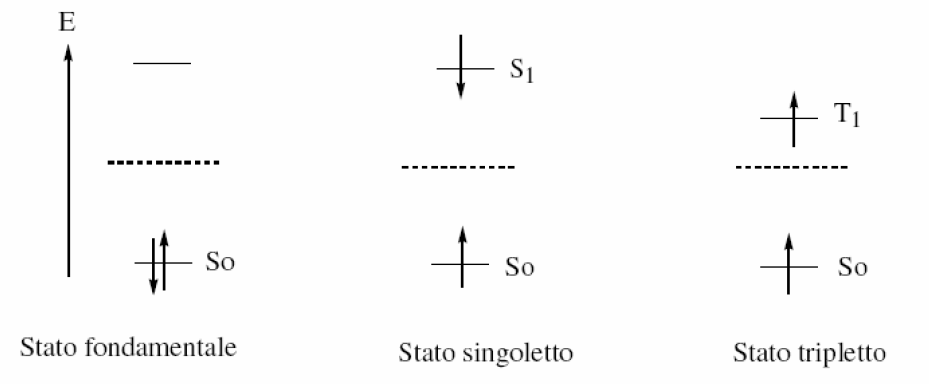
\includegraphics[scale=.40]{img/CAP1spin.png}
 \caption{\small{ Rappresentazione dei differenti stati elettronici. Lo stato fondamentale $S_0$ (sinistra), in seguito ad
eccitazione, può mutare nello stato di singoletto $S_1$ (centrale) o nello stato di tripletto $T_1$ (destra). }}
 \label{fig:spin}
\end{figure}

Per analizzare meglio i vari processi coinvolti nella diseccitazione bisogna fare riferimento al diagramma di Jablonski (\figurename~\ref{fig:jablonski}).
A seguito dell'assorbimento di luce (A), una molecola nello stato fondamentale ($S_0$) viene eccitata, per la conservazione dello spin, a uno dei suoi stati elettronici di singoletto ($S_1, S_2,\ldots$). 
L'energia vibrazionale della molecola eccitata viene trasferita a molecole vicine in seguito a collisioni e perciò vi è sempre un rapido ritorno al più basso livello vibrazionale dello stato di singoletto eccitato, senza emissione di radiazioni.
Questo fenomeno di rilassamento vibrazionale (R.V.) viene detto \textit{Conversione Interna} (C.I.) e si verifica in tempi dell'ordine di $10^{-12}$ s. 
C'è poi la possibilità che avvenga la \textit{Conversione di Sistema} (C.S.) o Intersystem Crossing, ossia che lo spin dell'elettrone, a causa degli urti con le altre molecole e dei moti molecolari, si inverta, comportando perciò il passaggio dallo stato di singoletto ($S_1$) allo stato di tripletto ($T_1$). 
La radiazione fluorescente (F) è generata da transizioni tra stati con la stessa molteplicità di spin (es. $S_1 \to S_0$). 
Nella fosforescenza (P), al contrario, la transizione coinvolta comporta sempre la variazione della molteplicità di spin (es. $T_1 \to S_0$).

\begin{figure}
 \centering
 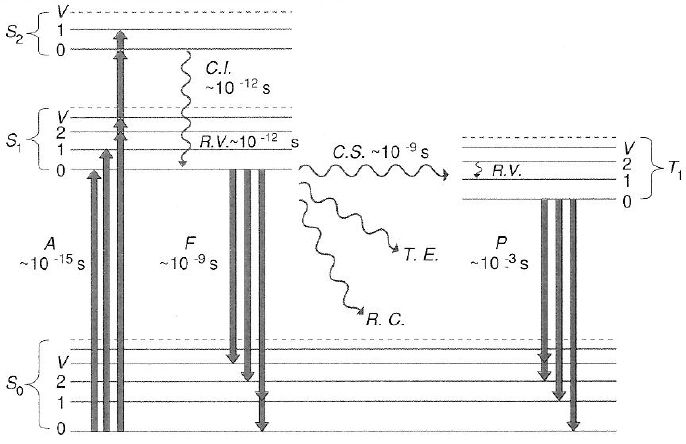
\includegraphics[scale=.45]{img/CAP1jablonski.JPG}
 \caption{\small{Diagramma di Jablonski. Nello schema $S_0$ indica il livello di energia elettronica fondamentale; $S_1$ ed $S_2$ sono rispettivamente il primo ed il secondo livello elettronico eccitato di singoletto; $T_1$ è il primo livello di tripletto. Sono indicati anche i sottolivelli di energia vibrazionale, in ordine di energia crescente, con $V_0, V_1, ...$, mentre non sono rappresentati i sottolivelli rotazionali.}}
 \label{fig:jablonski}
\end{figure}

I parametri tipici della fluorescenza sono:
\begin{description}
\item [Tempo di vita:]
Esso è definito come tempo medio di permanenza della molecola nello stato eccitato e per la fluorescenza è solitamente dell'ordine dei nanosecondi.
\item [Trasmittanza:]
Essa è definita, tramite la legge di Lambert-Beer, come rapporto tra l'intensità della luce trasmessa attraverso un mezzo di spessore s e l'intensità incidente: $$ T=\frac{I}{I_0} = e^ {k_\lambda s}$$ dove $k_\lambda$ è detto \textit{coefficiente di estinzione} ed è un parametro dipendente dal mezzo e dalla lunghezza d'onda della luce incidente.
\item [Efficienza quantica o resa:] 
Essa è definita come il rapporto tra il numero di fotoni emessi rispetto a quelli assorbiti. 
Questo coefficiente può assumere un valore compreso tra 0 (molecola non radiativa) e 1. I fluorofori hanno una resa quantica tipicamente non superiore a 0.1 per evitare fenomeni di re-emissione\cite{quantumyield}.
\end{description}


\subsection{Meccanismi di fading}

Esistono casi in cui la fluorescenza di una molecola può essere ridotta di intensità o addirittura annullata. 
Il termine che si usa per descrivere tale fenomeno è \textit{fading}, a sua volta distinguibile in quenching e photobleaching.
Entrambi i processi riducono il valore della resa quantica e il tempo di vita della fluorescenza.

\subsubsection*{Photobleaching}
Il meccanismo del photobleaching è dovuto a reazioni fotochimiche, provocate dalla luce di eccitazione, che variano in modo irreversibile la composizione del fluorocromo, rendendolo non più fluorescente. 

Tale fenomeno è oggi ancora poco conosciuto.
Esso coinvolge infatti molti fattori e può differire da un campione all'altro o anche da parti distinte di uno stesso.
L'assorbimento di luce comporta l'aumento del numero di molecole nello stato eccitato; essendo questo molto più reattivo di quello fondamentale, si ha che una piccola ma significativa frazione di molecole si trova coinvolta in nuove reazioni fotochimiche, a discapito dell'emissione di fluorescenza. 
Tali reazioni avvengono per lo più con ossigeno molecolare e causano la produzione di nuove molecole, che possono essere non-fluorescenti o addirittura incapaci di assorbire la luce incidente.
Ovviamente la quantità di photobleaching dipende dall'intensità della luce di eccitazione e risulta variabile durante il periodo di illuminazione: nei primi millisecondi di irraggiamento non è presente, successivamente aumenta in modo molto veloce per pochi secondi ed infine continua a procedere  più lentamente, andando ad attenuarsi.

Per ristabilire le proprietà fluorescenti del fluoroforo si può privare il campione della luce, mentre mantenuto a basse temperature. 
Inoltre, per evitare direttamente il fenomeno di photobleaching si può sfruttare un impulso di eccitazione molto breve o un fluorocromo particolarmente fotostabile.

Il fenomeno del photobleaching può essere anche indotto volontariamente per studiare il recupero di fluorescenza in un certo campione. 
Tale tecnica prende il nome di \textit{Fluorescence Recovery After Photobleaching} (FRAP) (\figurename~\ref{fig:FRAP}).

In particolari casi, sottoporre il campione alla luce di eccitazione per periodi prolungati può comportare un effetto totalmente opposto al photobleaching, detto \textit{photoactivation}. 
Difatti la manifestazione di tale fenomeno fa sì che la fluorescenza osservata, anzichè diminuire con il crescere del tempo di esposizione, aumenti rispetto al livello inizialmente mostrato. 
Nel caso in cui le cellule coinvolte siano cellule vitali, questo fenomeno può produrre effetti tossici molto dannosi.

\begin{figure}
 \centering
 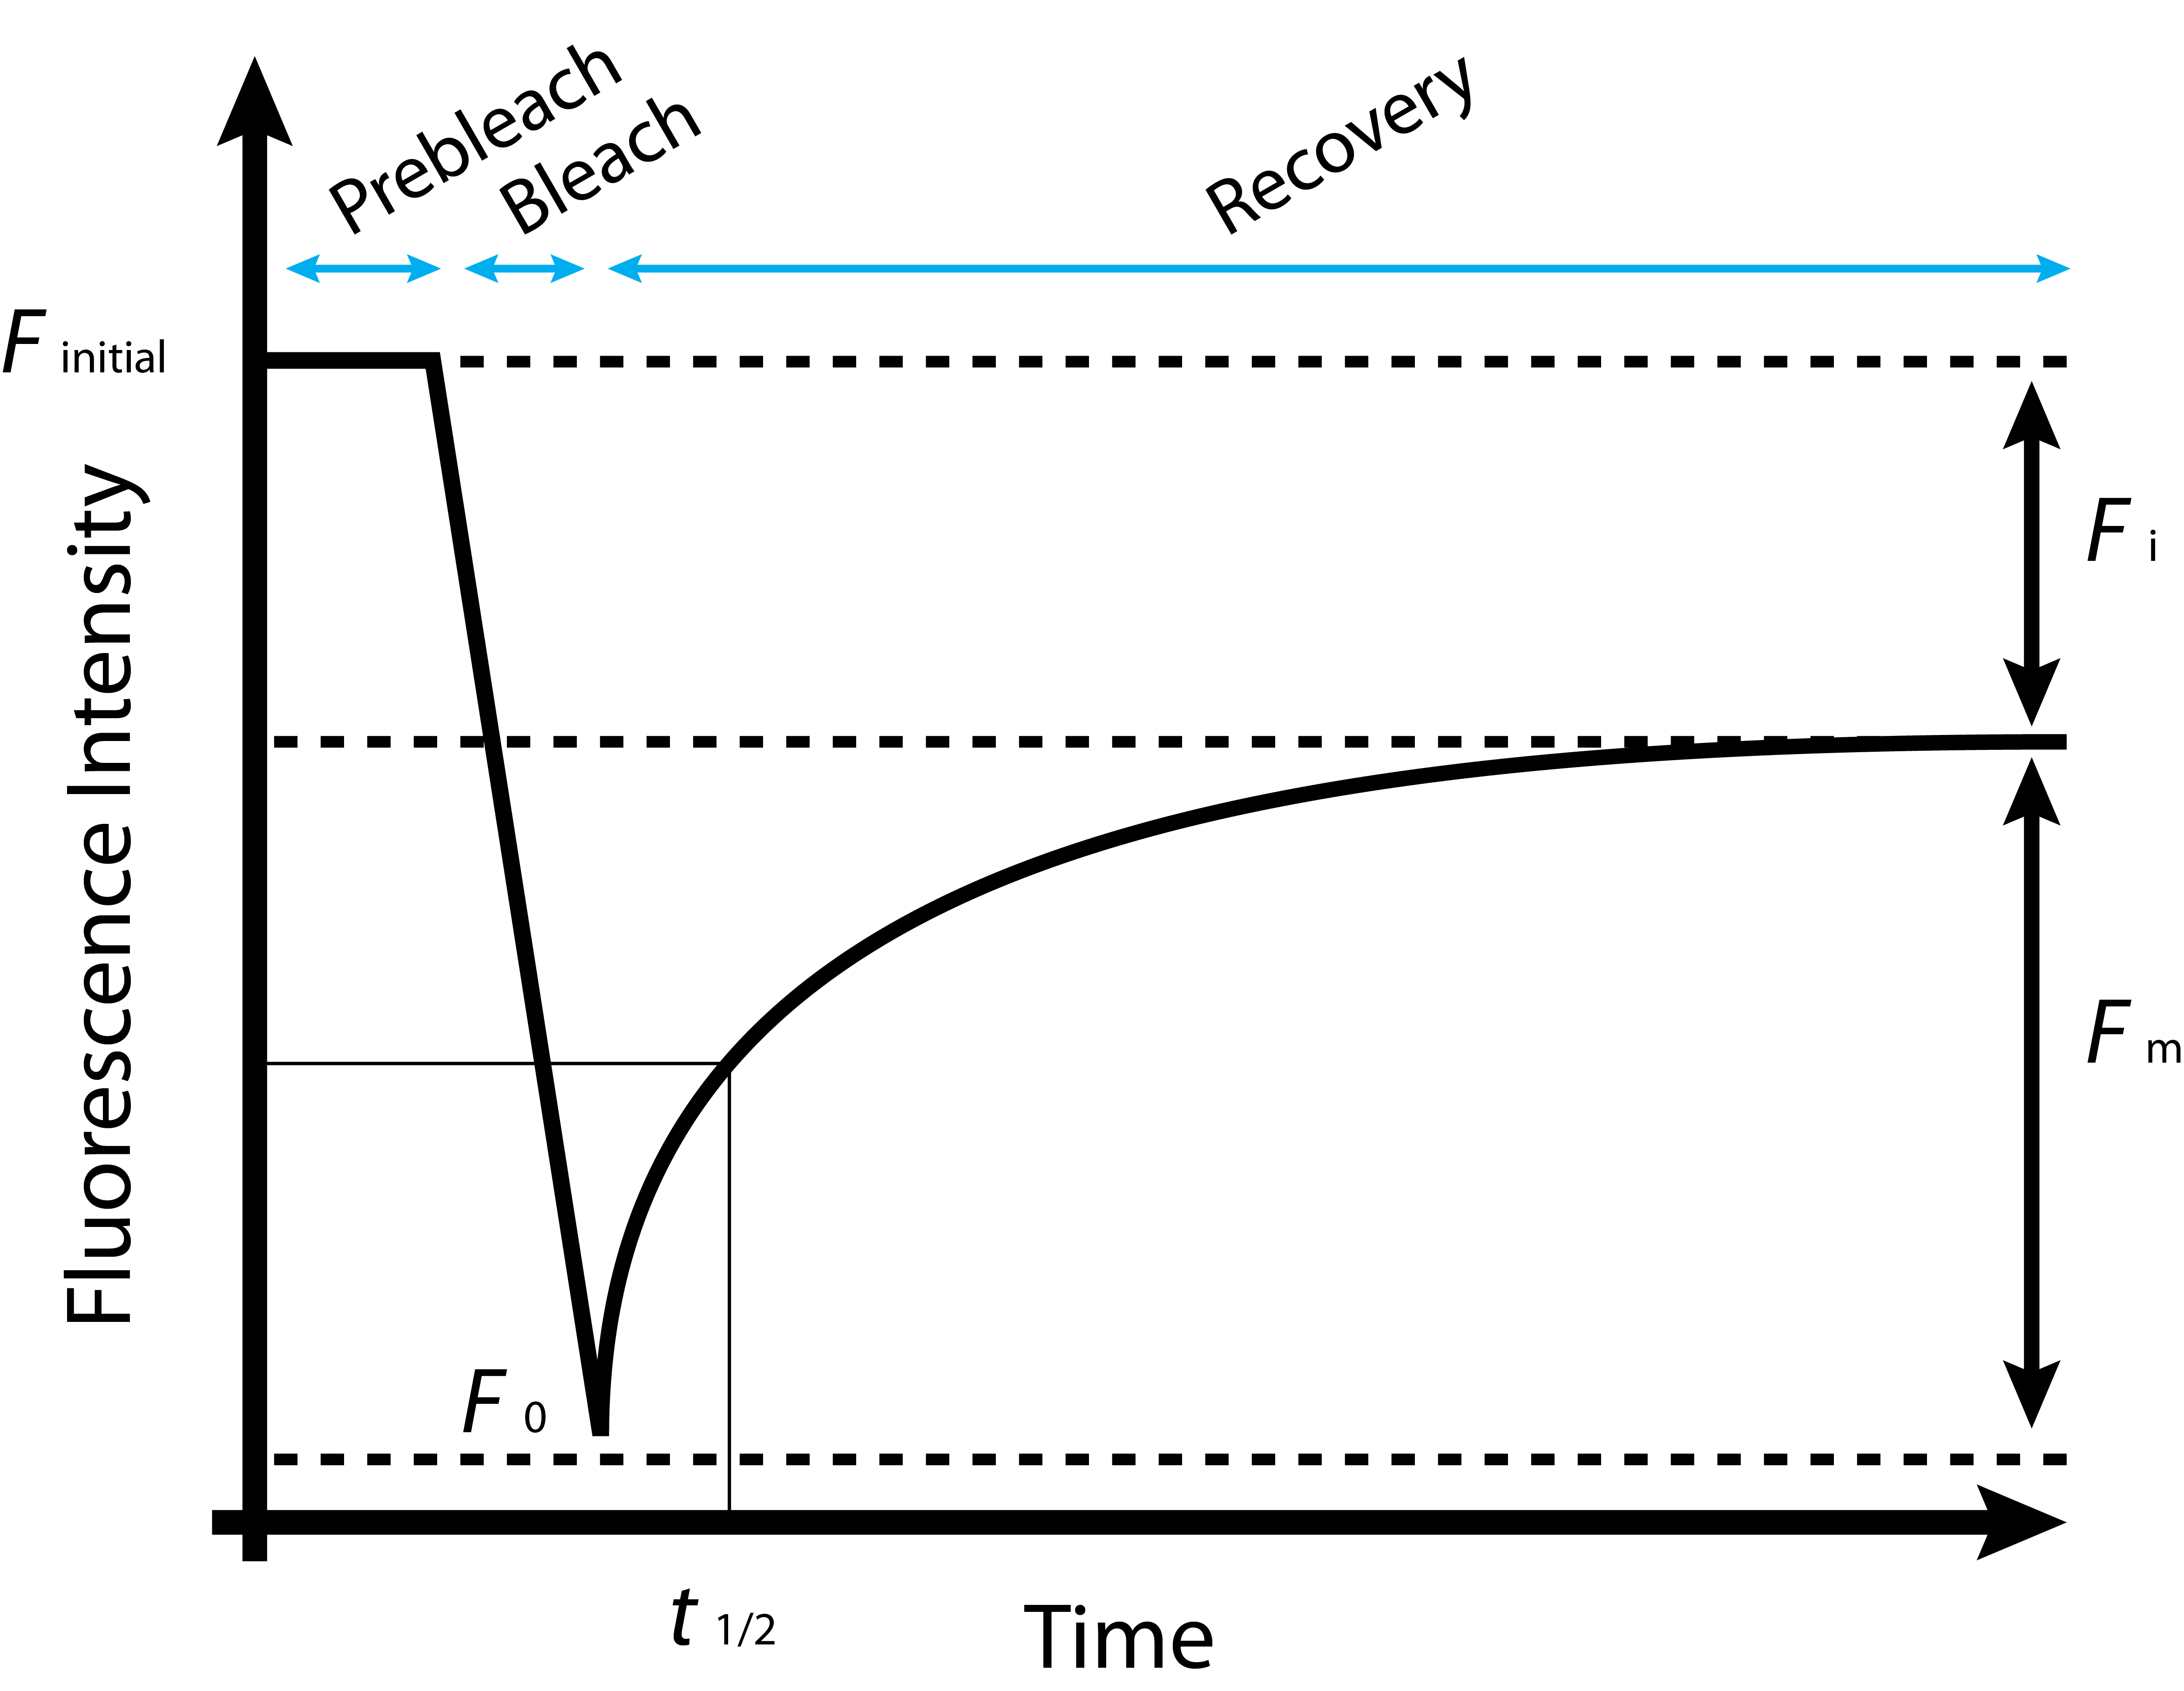
\includegraphics[scale=1]{img/CAP1FRAP.png}
 \caption{\small{Curva del FRAP. $F_{initial}$ ed $F_0$ sono rispettivamente l'intensità di fluorescenza antecedente ed immediatamente successiva al photobleaching; $F_m$ ed $F_i$ sono rispettivamente la frazione mobile ed immobile, ossia la frazione che contribuisce o no al recupero; $t_{1/2}$ è il tempo di recupero di metà frazione mobile.}}
 \label{fig:FRAP}
\end{figure}

\subsubsection*{Quenching}
Il meccanismo di quenching è dovuto alla presenza di molecole nel sistema, le quali comportano un processo di disattivazione in grado di ridurre la fluorescenza. Vengono solitamente distinti quattro tipi di quenching \cite{quenching}:
\begin{description}
\item [Quenching da temperatura:]
La fluorescenza decresce all'aumentare della temperatura dall'1\% al 5\%, a seconda del campione in esame. 
La causa è probabilmente da associare all'aumento di energia cinetica, quindi all'incremento delle collisioni molecolari, che provoca una maggior probabilità di transizione non radiativa verso lo stato fondamentale.

\item [Quenching da impurità o dinamico:]
La fluorescenza può diminuire o aumentare a causa della presenza di altre molecole nel mezzo.

Una molecola eccitata può trasferire il suo eccesso di energia ad una molecola adiacente che passa quindi nel suo stato eccitato, da cui potrà decadere
secondo ognuno dei meccanismi descritti precedentemente. 
Se l'accettore è non-fluorescente si avrà come risultato un fenomeno di quenching. 
Dato che il trasferimento di energia dal marcatore all'impurità può essere molto efficiente e può aver luogo fino a distanze di un micrometro, una concentrazione molto piccola di impurità può produrre un alto valore di quenching. 
Uno dei quenchers più noti è l'ossigeno molecolare che causa una grande riduzione nella fluorescenza, sino ad annullarla completamente. 
Ciò può essere evitato introducendo nel mezzo di coltura un agente riduttivo.
D'altra parte può anche accadere che l'accettore sia fluorescente ed in tal caso la luminescenza risulta incrementata dalla presenza dell'impurità.

Quest'ultimo tipo di quenching dinamico può essere sfruttato in modo positivo, per esempio nella cosiddetta \textit{F\"{o}rster Resonance Energy Transfer} (FRET o FET). 
Essa consiste nel trasferimento dell'eccitazione di una molecola donatrice ad una accettrice attraverso un processo non radiativo di interazione dipolo-dipolo.
La FRET ha varie caratteristiche: varia come $1/R^6$ e di conseguenza dipende strettamente dalla distanza donatore-accettore ($R$) che deve essere al più dell'ordine di $10\ nm$; necessita la sovrapposizione dello spettro di emissione del donatore con quello di eccitazione dell'accettore; dipende dall'orientazione relativa dei momenti di dipolo di transizione delle due molecole.
\item [Quenching statico:]
Esso si verifica quando le molecole del donatore e dell'accettore si trovano nello stato fondamentale, invece che in quello eccitato, e si legano insieme a formare un'unica molecola, anch'essa nello stato fondamentale ma non più fluorescente, avente un unico spettro di assorbimento. 
La causa è spesso legata ad effetti di idrofobia, ossia le due molecole si uniscono insieme per minimizzare il contatto con l'acqua.
\item [Quenching da concentrazione:]
Normalmente con l'aumentare della concentrazione del fluorocromo aumenta la quantità di fluorescenza. 
Tuttavia a concentrazioni molto elevate interviene il cosiddetto quenching da concentrazione, che comporta una riduzione della fluorescenza.
Questo può avvenire per aggregazione delle molecole del fluorocromo (come ad esempio nelle porfirine) oppure per trasferimento non radiativo di energia fra molecole identiche.\todo{vedi le general FAQ di prsbio.com}
\end{description} 


\section{Sonde fluorescenti}

Sia nel mondo vegetale che nel mondo animale, diverse sostanze naturali manifestano una fluorescenza intrinseca, detta anche \textit{autofluorescenza}.
Ne sono esempi le clorofille, molti pigmenti naturali (in particolare quelli di natura lipidica), alcuni amminoacidi (es. triptofano e tirosina), molti enzimi, coenzimi (es. NAD e NADH), cofattori (es. FAD e FADH) e molecole aromatiche. 
Tuttavia la maggior parte delle molecole biologiche di interesse biofisico non sono autofluorescenti all'interno degli intervalli spettrali sfruttati e anche quelle che lo sono, in genere, non possono essere distinte tra loro sulla base della loro fluorescenza intrinseca.

Per ovviare a ciò, Max Haitinger nel 1933 introdusse l'uso della fluorescenza secondaria nello studio dei preparati biologici, ossia aggirò tale problema utilizzando dei marcatori esterni, detti comunemente sonde o \textit{probes} fluorescenti. 
Da allora la procedura comunemente usata in microscopia è quella di marcare gli elementi che si vogliono studiare con fluorofori, che si legano a target specifici delle molecole di interesse, le quali, dopo opportuna eccitazione, potranno essere selettivamente rivelate grazie al segnale luminoso emesso dalle sonde. 

Ovviamente introdurre un agente esterno all'interno di un componente biologico non è così banale, infatti bisogna fare in modo che rispetti tutte le esigenze della cellula: il marcatore deve raggiungere il target e non allontanarsi da esso durante l'intera rilevazione; una volta \textit{in situ} il probe idealmente si deve comportare come un agente passivo che non induce perturbazioni significative nelle strutture o nelle funzioni biologiche che si vogliono studiare; infine si deve cercare di evitare che tramite il processo di misura si creino effetti negativi come fading e fototossicità.

I primi fluorofori usati erano semplici coloranti, perciò non specifici, e per questo si legavano a costrutti presenti praticamente ovunque nella cellula, producendo un segnale molto diffuso. 
Poi, con l'avanzare delle conoscenze biochimiche si trovarono sonde organiche, inorganiche o chimiche in grado di marcare costrutti molto specifici all'interno della cellula (es. nucleo, membrana, mitocondri, etc) e si introdussero protocolli sperimentali adeguati. 
La tecnologia attuale permette persino di sfruttare fluorocromi in grado di marcare solo particolari ioni, come ad esempio $Ca^{2+}$, $Mg^{2+}$, $Na^{2+}$, $Cl^-$ ed $O_2$.

Le proprietà che caratterizzano maggiormente i marcatori fluorescenti sono:
\begin{itemize}
\item Spettri di eccitazione ed emissione, importanti per la scelta del fluoroforo più adatto al proprio apparato sperimentale. 
Il primo si sceglie in modo da essere il più possibile centrato sulla lunghezza d'onda emessa dalla sorgente di luce, mentre il secondo deve poter essere rilevabile dagli strumenti a disposizione. 
\item Efficienza quantica, per avere il miglior segnale in fluorescenza rilevabile con i rivelatori utilizzati. 
\item Affinità con i diversi costrutti molecolari e tessuti subcellulari.
\item Modalità con cui possono penetrare all'interno della cellula.
\end{itemize}
Perciò, per la scelta del protocollo sperimentale atto alla marcatura, è fondamentale analizzare le specifiche dei vari coloranti, disponibili su database online. 
In \tablename~\ref{TABfluo} ne vengono riportati alcuni di uso comune.

\begin{table}[!ht]
 \begin{center}
\begin{small}
\begin{tabular}{lcc}
\hline\hline
\textbf{Colorante}&\textbf{Eccitazione}&\textbf{Emissione}\\
&\textbf{\small{(nm)}}&\textbf{\small{(nm)}}\\
\hline
\textbf{Fluorofori comunemente impiegati}&&\\
Fluoresceina-5-isotiocianato (FITC)&496&518\\
Isotiocianato di tetrametilrodamina (TRITC)&550&570\\
Tetrametilrodamina&554&576\\
Lissamina rodamina&572&590\\
Rosso Texas&592&610\\
\hline
\textbf{Coloranti per il nucleo}&&\\
4',6'-Diamidino-2-fenilindolo cloridrato (DAPI)&359&461\\
\hline
\textbf{Indicatori di calcio}&&\\
Indo-1&380&400/475\\
Fluo-2&340/380&510\\
Fluo-3&506&526\\
\hline
\textbf{Molecole reporter}&&\\
Proteina fluorescente verde (GFP)&395/475&509\\
DsRed&558&583\\
\hline
\textbf{Coloranti per i mitocondri}&&\\
Rodamina 123&507&529\\
\hline\hline
\end{tabular}
\caption{\small{Caratteristiche dei fluorofori di uso comune.}}
\label{TABfluo}
\end{small}
\end{center}
\end{table}


\subsection{Tecniche di marcatura}

Dall'analisi delle proprietà dei vari fluorocromi sono nate cinque principali tecniche specifiche di marcatura \cite{tecniche}:
\begin{enumerate}
\item tecnica di marcatura con coloranti fluorescenti;
\item tecnica di immunofluorescenza;
\item tecnica dell'ibridazione fluorescente in situ (FISH);
\item tecnica di marcatura con proteine fluorescenti;
\item Quantum Dots (QD).
\end{enumerate}

\subsubsection*{Marcatura con coloranti fluorescenti}
Nella tecnica di marcatura con coloranti fluorescenti le sonde sono assorbite direttamente dalla cellula, sfruttando solitamente i gradienti di concentrazione o il potenziale di membrana, ed in questo modo esse si concentrano in zone intracellulari specifiche.
Con tale metodo è possibile anche eseguire misure quantitative delle cellule vive che hanno assorbito il colorante fluorescente, dato che appaiono intensamente colorate su sfondo scuro. 

\subsubsection*{Immunofluorescenza}
La tecnica di immunofluorescenza si basa su anticorpi legati chimicamente a fluorofori, così da sfruttare successivamente il legame altamente specifico anticorpo-proteine. 
Dato che gli anticorpi sono molecole che si legano selettivamente a specifiche parti della cellula, in tal caso non sarà più il fluorocromo a decidere il legame, ma direttamente la molecola biologicamente attiva.

Questo metodo presenta come vantaggio il poter ottenere informazioni molto precise sia dal punto di vista spaziale che della specificità del legame, a discapito di dell'intensità, che risulta in tal caso debole a causa della piccola quantità di colorante legato.
Tuttavia il segnale può essere amplificato utilizzando la tecnica di \textit{immunofluorescenza indiretta}: un anticorpo specifico non marcato, detto anticorpo primario, diviene target di numerosi anticorpi secondari marcati da uno specifico fluoroforo. 
Solitamente per tale scopo si sfruttano come coloranti la fluoresceina, che emette nel verde se eccitata con luce blu, e la rodamina, che emette nel rosso se eccitata con luce giallo/verde.

\subsubsection*{Ibridazione fluorescente in situ}
La tecnica dell'ibridazione fluorescente in situ (FISH, \textit{Fluorescence In Situ Hybridization}) sfrutta probes che si legano in modo estremamente selettivo ad alcune regioni del cromosoma. 
Tale metodo permette di rilevare e localizzare la presenza/assenza di specifiche sequenze di DNA.

\subsubsection*{Marcatura con proteine fluorescenti}
La tecnica di marcatura con proteine fluorescenti sfrutta tecniche di ingegneria molecolare, in grado di modificare geneticamente una cellula eucariote rendendola capace di produrre una proteina fluorescente, ma senza alterarne la sua normale funzionalità. 
In questo modo la proteina marcata può essere sfruttata come tracciante (oltre che marcatore), ossia può essere seguita nel corso della sua sintesi, dalla compartimentazione intracellulare sino alle interazioni con le diverse strutture cellulari.

Il fatto che le proteine fluorescenti possano essere fuse alla proteina d'interesse così da rendere il targeting molto preciso è un grande pregio rispetto ai coloranti organici. 
I vantaggi di questo metodo biomolecolare sono soprattutto il non avere bisogno di tecniche invasive per visualizzare in cellule vive una proteina oggetto di studio, a differenza di quel che accade per esempio nella tecnica di immunofluorescenza dove le cellule devono essere precedentemente fissate; l'assenza di problemi di loading del fluoroforo, di rumore di fondo, di interazioni tra colorante ed ambiente circostante e tra le stesse molecole di fluoroforo ed infine l'alta precisione del targeting in quanto la proteina è prodotta dalla cellula stessa. 
Le difficoltà risiedono invece per lo più nell'ottimizzazione delle tecniche di trasfezione, attraverso cui la cellula viene geneticamente modificata, così da produrre la proteina di interesse.

Tra le più famose proteine fluorescenti vi sono la \textit{Green Fluorescent Protein} (GFP), isolata dalla medusa ``Aequorea Victoria'', e la \textit{Red Fluorescent Protein} (RFP), isolata dal corallo ``Discosoma'' (\figurename~\ref{fig:proteine}). 
La fluorescenza intrinseca di queste proteine è dovuta alla presenza di triptofano.

\begin{figure}
 \centering
 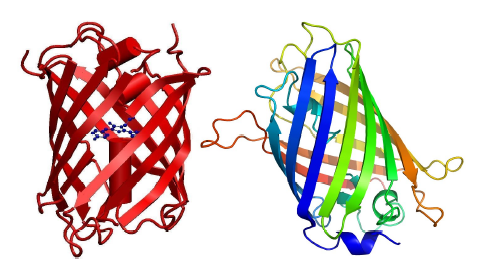
\includegraphics[scale=.50]{img/CAP1proteine.png}
 \caption{\small{ Struttura tridimensionale della RFP (sinistra) e della GFP (destra).}}
 \label{fig:proteine}
\end{figure}

\subsubsection*{Quantum Dots (QD)}
I Quantum Dots (QD) sono una classe di fluorocromi sviluppata negli ultimi anni sulla base di nuove competenze in ambito nanotecnologico.
Essi sono costituiti da un nucleo semiconduttore di cadmio-selenio ($ CdSe $) ricoperto da uno strato di solfato di zinco ($ ZnS $), necessario per migliorare l'efficienza quantica e la fotostabilità. 
Questi nanocristalli hanno dimensioni comparabili con le proteine (es. GFP) e, se eccitati ad opportune lunghezze d'onda, emettono fluorescenza, in colori differenti a seconda della dimensione della loro struttura (\figurename~\ref{fig:QD}).  
Infatti è il diametro del nucleo semiconduttore che determina lo spettro di emissione del QD: all'aumentare della dimensione si ha un aumento della lunghezza d'onda. 
Ciò è dovuto al fatto che QD più grandi presentano livelli di energia più vicini tra loro, così da poter assorbire anche i fotoni meno energetici ed emettere a grandi lunghezze d'onda. 

\begin{figure}
 \centering
 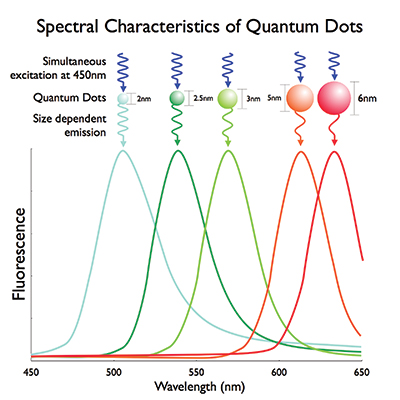
\includegraphics[scale=.60]{img/CAP1QD.jpg}
 \caption{\small{ Dimensione dei QD in relazione alla lunghezza d'onda di emissione.  I QD assorbono luce ad energia maggiore (lunghezza d'onda minore) e la convertono in luce ad energia minore (lunghezza d'onda maggiore). Monitorando la produzione dei Quantum Dots è possibile far sì che essi emettano luce ad ogni lunghezza d'onda dello spettro del visibile.}}
 \label{fig:QD}
\end{figure}

Un pregio di questa classe di fluorofori è legato agli spettri di eccitazione e di emissione: il primo risulta pressoché continuo e molto ampio, mentre il secondo è particolarmente piccato e simmetrico. 
In tal modo è possibile l'eccitazione di diverse specie di QD utilizzando un'unica fonte luminosa per la fluorescenza multipla, senza sovrapposizioni di segnale.
I QD emettono una fluorescenza circa 20 volte maggiore rispetto ai coloranti organici, la loro luminescenza ha lunga vita media ($30-100\ ns$) e presentano, grazie alla loro natura inorganica, l'ulteriore vantaggio di non subire photobleaching ossidativo, presente invece per i coloranti organici e le proteine fluorescenti. 
Tali proprietà diminuiscono le interferenze con l'autofluorescenza di background, rendendo i Quantum Dots molto utili nella monitorizzazione in continuo dei fenomeni biologici. 

Dato che le proprietà luminescenti dei QD ``nudi'' sono molto sensibili a vari tipi di interazione, si usa ricoprirli con materiali inorganici, solitamente solfato di zinco, che avendo un maggiore gap tra i livelli energetici migliorano le capacità luminescenti anche più del 50\% ($(CdSe)ZnS$ core-shell QDs).
Sotto questa forma però i QD non risultano biocompatibili e perciò è necessario sintetizzarli in presenza di composti idrofobici e inorganici, come l'ossido di trioctilfosfina (TOPO). 
In questo modo la loro superficie viene avvolta con una lunga catena alchilica, così da renderli solubili in solventi non polari, come il toluene. 

Una difficoltà riscontrabile con i QD è la loro traslocazione all'interno della cellula. 
Tuttavia questo problema è stato in parte risolto mediante l'utilizzo di proteine di trasporto, il cui compito naturale è appunto quello di trasportare altre proteine dall'esterno all'interno della cellula grazie alle loro forti cariche positive.

I QD sembrano dunque essere la futura tecnologia per lo studio di alcuni processi dinamici intracellulari, come per esempio il tracciamento delle proteine recettore e la loro distribuzione nello spazio e nel tempo.
